%update: more Dec28
%note: image 4waysprobe is not here

\begin{savequote}[75mm] 
We become what we behold. We shape our tools, and thereafter our tools shape us.
\qauthor{Marshall McLuhan} 
\end{savequote}

\chapter{Engineering of Probing Techniques inside TEM}

\newthought{We are not satisfied with the limited possibilities provided by TEM}, and we are eager to introduce more variable to the system because that's how we see dynamics in the real applications.
In the following subsections, I will firstly introduce how we cooperate chemicals, light, mechanical manipulations and electrical interaction to the microscopy. 
Especially for the new optical fiber compatible TEM, where all the four factors could be included, the inside and outside part of the \emph{in situ} microscopy is detailed described. 
Finally we will take a look at the what the system can do and its short-backs. 

%before us, stm tem holder
\section{Introducing chemicals, electricity, strain into the microsocpe}

As we discussed in Chapter 1, \emph{in situ} microscopy does introduce parameters such as heat, cooling, gas, liquid, etc. to the system, but now we focus on how we introduce these variables in the delicate microscope. In most cases, {\em in situ} microscopy are performed by specially designed TEM holders, such as heating holder equiped with heating electrical wire or MEMS microheater. At the same time, some researchers make adaptions on microscope to introduce the variables. In my Ph.D. research, expect electron beam, four more variables are introduced: chemicals (solid), mechanical probing, electrical contact and optical access. \\

For electrical biasing, many TEM holders are commercially available. This holder provides a combination of TEM and Scanning Tunneling Microscopy(STM) techniques, which are used simultaneously in one instrument for the TEM characterization, STM imaging, introducing chemicals and electrical mesurements. The STM probe scanner have a very wide range of motion from picometers to millimeters, which is employed either for a coarse adjustment of the sample orientation, or a precise probe positioning. \\

Electrical contacts with nanoscaled interfaces can be realized at will by precise positioning the movable probe in the desired spot, enabling simultaneous investigating of the specimen’s structural and electronic conduction properties with the optional strain or chemicals.\\

If the electrical biasing is realized by piezo probing, we can also ultilize the probe for introducing chemical (solid on probe) and mechanical strain (without force value measurement\footnote{It is possible to combine atomic force microscopy into TEM holder to introduce mechanical measurements, but the probe cannot be used for electrical biasing anymore.}). \\

I briefly discussed the ways to input chemical, electrical biasing and mechanical factors in TEM; However, introducing the other factor -- light -- to the system is challenging. Therefore I will discuss this part, which is very good reference for future research, in next section. 

\section{Introducing light into the microscope}
\subsection{Previously}
Introducing the other factor -- light -- to the system while at the same time maintain the other factors is very tricky. Some researchers and companies tried to introduce light without probing. This means that no introduce of chemicals, electricity and mechanics. We may first investigate how they introduce/collect light to/from the microscope. 
Table \ref{table2.1} compare the two possible ways to implement light into the system. 

\begin{table}[ht]
\centering 
\begin{tabular}{|c|c|} 
\hline 
by adaption on microscope & by using special holder \\ [0.5ex] 
\hline 
light plane different from specimen & on same plane with specimen \\[1.5ex] 
require take off detector/aperture & a specially designed holder \\[1.5ex]
optics can be realized by lens on bench & only optical fiber\footnote{For the moment only optical fiber, but it is possible to have lens system inside the holder, please read chapter 7 for more information.} \\[1.5ex]
complicated, high power, high cost & no addaption to TEM\\[1.5ex]
\hline
\end{tabular}
\caption{Two main ways to implement light into a TEM} 
\label{table2.1} 
\end{table}

As shown in the table, by replacing an aperture or making a window for optical path locate the light path tilted. The light goes trough the microscope shell at different level from the specimen plane. In some cases, it is possible to replace a detector or an aperture by desired modules to provide variables. As shown in Figure \ref{fig:2_1} With a certain angle, the light can hit the specimen. The system could be very complicated if optics are realized by lens system on optical bench including light sources, lens system and options such as CCD camera, chopper and monochromator. The system can be very powerful if the optical system on table is well designed and precisely assembled. However, the cost of time and funding is also expected to be significant. \\

\begin{figure}  
\centering
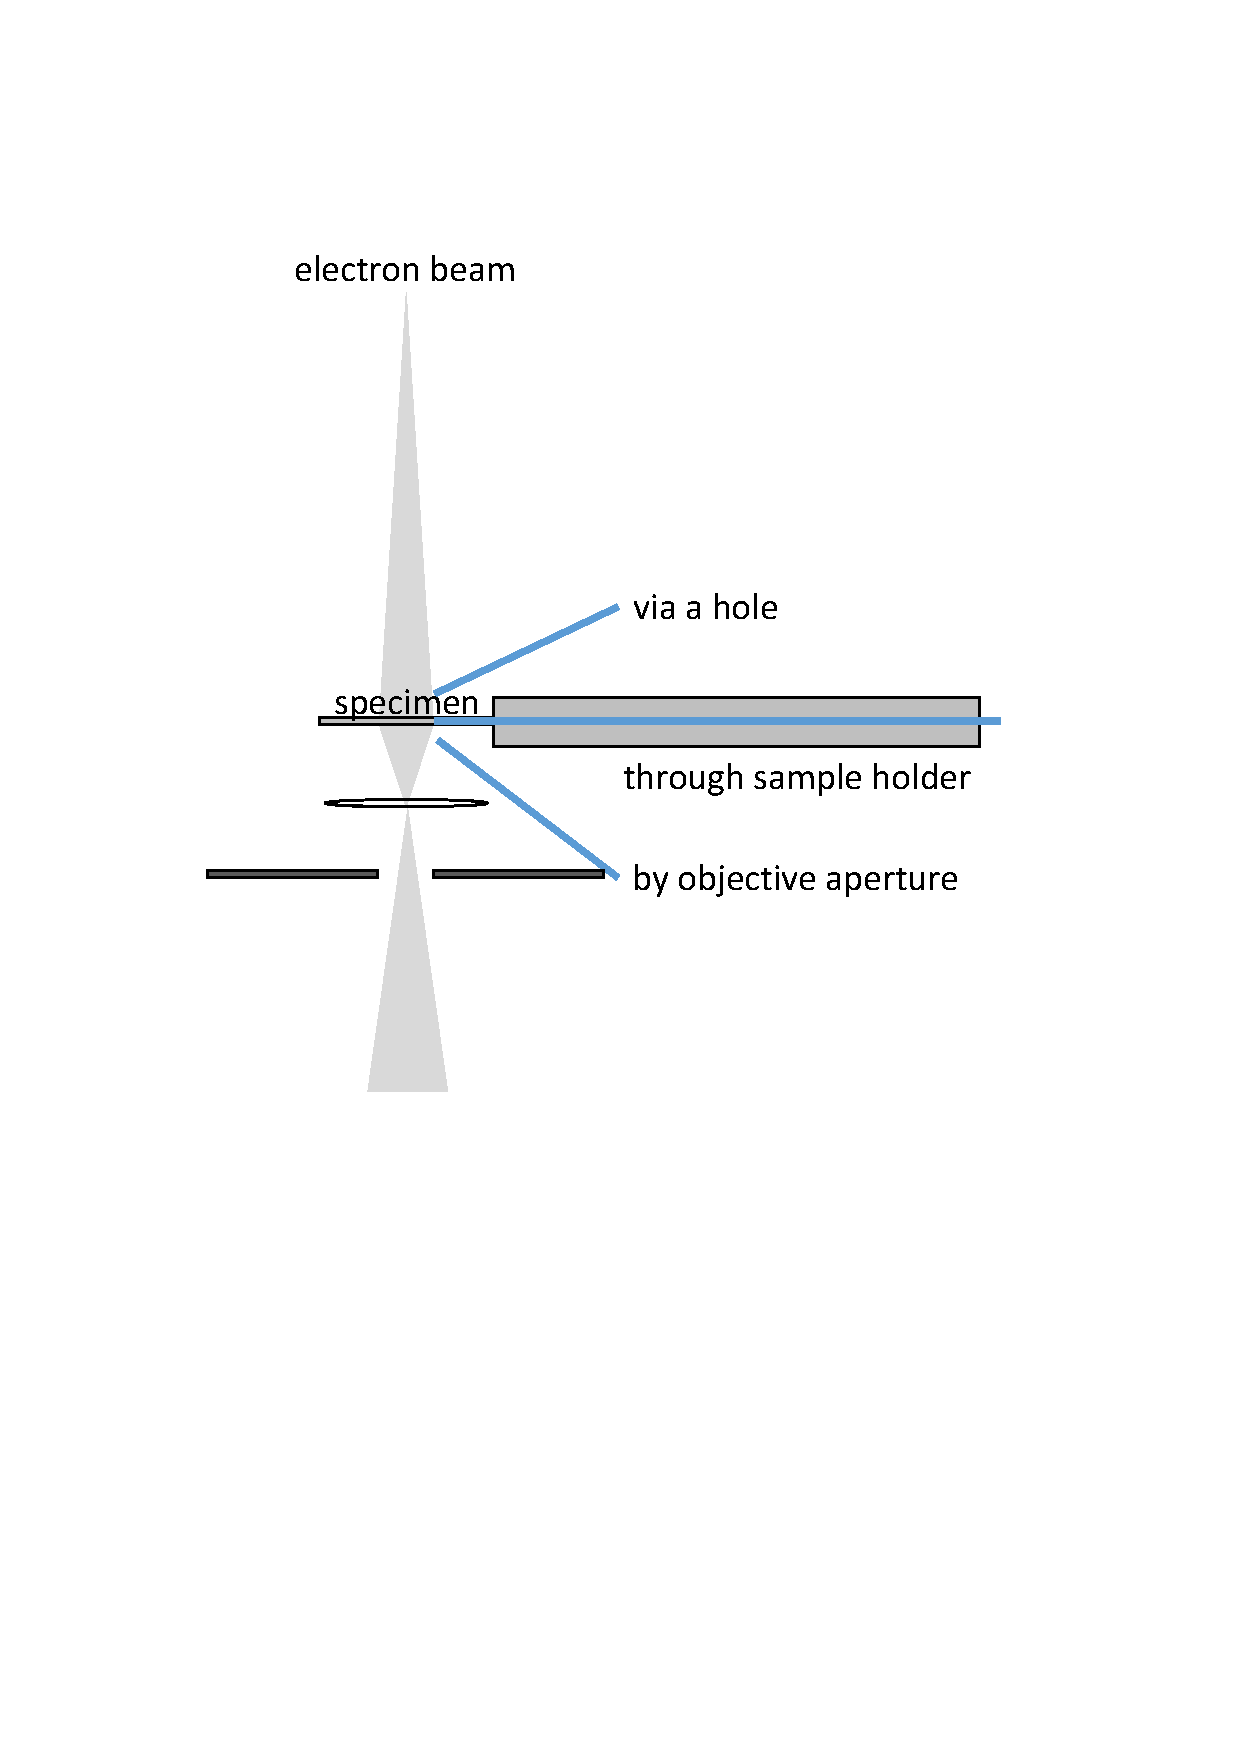
\includegraphics[width=270pt]{figures/figure2_1}
\caption[To put light into TEM.]{How light is compatible to TEM.
\label{fig:2_1}}
\end{figure}

For a special optical holder, the way is to install an optical fiber through the holder, as shown in Figure \ref{fig:2_1}, the light will be shinning on the specimen at about 90 degrees to the electron beam. In most cases, the microscope is owned by many users for various applications, and therefore the approach of using special optical holder is more practical -- it's quite luxury to drill a hole and install a optical bench on the microscope with everybodies' permission. 

A few groups have tried to take light into TEM. \\

Muto et al. (Kyushu University) managed to install optical fiber trough a 2 mm hole at an angle of 45 degrees.\cite{Tanabe2002,Furumoto2013} They manufactured the prototype of TEM-CL system with the light collecting parts integrated on the holder, but no parabolic reflector within the pole piece. The system is able to take cathodoluminescence(CL), X-ray emission spectroscopy and Electron Energy Loss Spectroscopy(EELS) at the same time, even with large angle sample tilt. The main disadvantage of the holder was a significant background level from the thermal glow of the electron gun and the CL signal of optical fiber. Later, Muto et al. and staff from {\em Nanofactory Instruments} developed a prototype optical holder implemented with an optical fiber through holder, on the side of specimen. The reflectors and optical fiber are placed away from the TEM optical axis. The light-collecting solid angle is approximately 1.3 strad, approximately 100 times larger than that of their first generation prototype. The sample is mounted at the end of the metal wire, of which the position can be controlled to the focal point of the mirror by the piezo-driven manipulator. In years 2012-2013, a few groups, including us, got optical holder (beta version) from {\em Nanofactory Instruments}. \\

One of the group is in Brookhaven National Laboratory. Yimei Zhu et al. obtained prototype optical holder from {\em Nanofactory} which allows two optical fibers and several delicate mirrors to locate light beam to the specimen. 
The multimodal optical nanoprobe allows scientists to perform all the usual experiments done in a TEM in addition to those involving optical excitation and measurement of the sample, electrical measurements on the sample, STM and combinations of these measurements. They emphasized the ability to simultaneously measure optical and electrical properties of the sample at nanoscale.\cite{Zhu2012Multimodal}  The factors introduced are very similar to our case, but their serious problems are about the calibration of location of light spot, which is realized by the adjustment of the tiny mirror screws; also, they are not able to confirm the location of light spot. Therefore the system is not so practical. \\

Minor and Grigoropoulos et al. have implemented a {\em in situ} TEM monitoring technique to observe the crystallization of a-Si during high power pulsed laser irradiation by directly coupling laser into a TEM through a fiber-optic probe. By realizing a near-field
scanning optical microscopy (NSOM) fiber probe scheme, this technique opens up a wide variety of new characterization possibilities.\cite{Xiang2012}

Kociak et al. in Université Paris-Sud \cite{Zagonel2011} developed STEM-CL system on Nion microscope which also using optical fiber as light guide from the microscope column to the CCD camera outside the microscope. The light is collected by a specially designed mirror system of which the focus point is on specimen. This CL-STEM imaging can be applied to obtaining luminescence spectra and imaging ultrastructure simultaneously.\cite{DOI: 10.1039/c6nr01908k}

In another group, Miller in Prof. Crozier's group in Arizona State University replaced EDS detector (first version) or objective aperture (second version on FEI Titan microscope) by an optical fiber and its associates to shine light onto chemicals to observe dynamics of photochemistry.\cite{Miller2012} But the problem is that they are not sure about the location of light spot, because they cannot observe the optical fiber which is out of the specimen plane. 

To conclude, by introducing light into TEM, researchers are capable to observe dynamics of photochemistry or thermo-effects, to obtain high resolution CL with EELS and Dark field imaging simultaneously. As summarized in Talbe \ref{table2.2}, almost all groups used optical fiber for introducing light rather than lens system on bench, most groups does not offer probing contact capability. In my case (NIMS in table), I would like to reach all functions based on the optical holder. 

\begin{table}[ht]
\centering 
\begin{tabular}{|c|c|c|c|c|} 
\hline 
Institute & fiber & though & Probing contact & practical for\\ [0.5ex] 
\hline 
Nagoya U. & Yes & hole, holder direct & No & CL\\[1.5ex] 
BNL & Yes & holder by sides & Yes & N/A\\[1.5ex]
LBNL & Yes& holder direct & No & NSOM heating\\[1.5ex]
U. Paris-Sud & Yes & holder direct & No & CL-Map, NSOM\\[1.5ex]
ASU & Yes & detector/aperture & No & Photochem.\\[1.5ex]
NIMS & Yes & holder direct & Yes & all above\\
\hline
\end{tabular}
\caption{Compare of the groups who introduced light to TEM} 
\label{table2.2} 
\end{table}

\subsection{Our holder adaption}
In our system, the microscope is not modified at all, we are very much putting all dynamics through the specimen holder. I proposed 4 sed ways to add electrical access on the piezo-driven optical fiber based on the Nanofactory optical holder, as shown in Figure \ref{fig:4modes}. One way is to 
%%%%%%%%%%get the image!!

Considering the fact that attaching a probe onto the piezotube driven hat would enable more dynamics possible to our microscopy, I finally decided to chose the plan to drill hole on side of hat to attach a probe on while at the same time coating gold onto the fiber tip to reduce charging of fiber during electron beam exposure. 

For nanostructures, sampling is a little bit easier, the sampling can be attached to the gold wire tip by touching, pressing, dipping or dropping. For thicker samples, the specimens can be made by FIB technique on to a half grid. 


\subsection{Outside the microscope}
The individual coaxial wiring in the holder for each contact gives pA noise levels during these measurements, allowing to measure low currents in non-ohmic contacts.


\section{Applications and limitations}
\subsection{Applications}
 The interface morphology, the contact area and orientation, the material crystallography, all of these factors can be precisely determined with high resolution microscopy, while a bias and a light applied on sample and probe allows to measure the electronic and optoelectronic conductive state of the contact. 
 
On the opposite way, by collecting optical signal from specimen through optical fiber, spatial resolved CL information is measured to be correlated to the crystallography information. 
This means that the 

\begin{figure}  
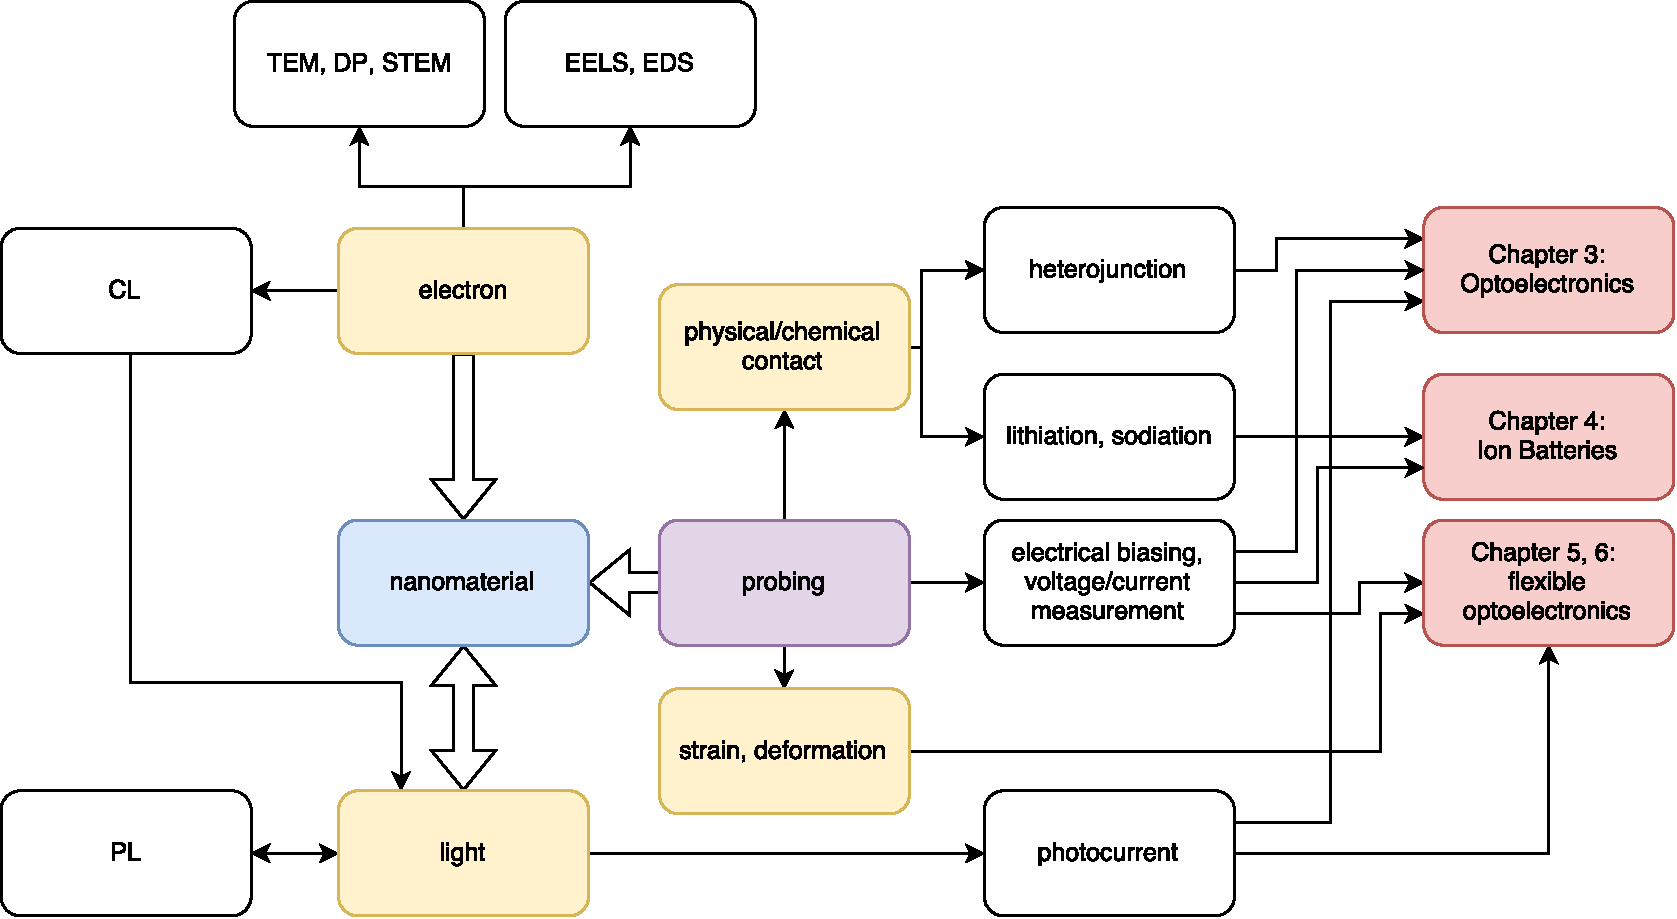
\includegraphics[width=400pt]{figures/figure2_apply}
\caption[Relationships between factors and applications.]{Relationships between factors and applications. Important dynamics are marked by yellow, some applications are marked by red, which will be detailed discussed in other chapters.
\label{fig:2_apply}}
\end{figure}

In Figure \ref{fig:2_apply}, the relationships between each factors are clearly presented. The applications of our light-compatible probing {\em in situ} TEM are not restricted to optoelectronics, flexible electronics/optoelectronics and lithium/sodium ion batteries, which are detailed discussed in chapters 3-6. More fields such as research topics on CL, PL, photovoltaic and photochemistry applications are expected to be explored. 


\subsection{Limitations}
First, the system is based on TEM, therefore most limitations of TEM also applied to our system; that is, the sampling requirement is high, the sampling efficiency is low, TEM imaging is 2D information, and electron beam may damage the specimen. 

